\chapter*{Introduction}
\label{ch:introduction}

\begin{chapquote}{Lewis Carroll, \textit{Alice in Wonderland}}
\enquote{But I don’t want to go among mad people,} Alice remarked. \enquote{Oh, you can’t
help that,} said the Cat: \enquote{we’re all mad here. I’m mad. You’re mad.} \enquote{How do
you know I’m mad?} said Alice. \enquote{You must be,} said the Cat, \enquote{or you wouldn’t
have come here.}
\end{chapquote}

In October 2018, Arjun Balaji asked the innocuous question,
\textit{What have you learned from Bitcoin?} After trying to answer this
question in a short tweet, and failing miserably, I realized that the things
I've learned are far too numerous to answer quickly, if at all.

The things I've learned are, obviously, about Bitcoin - or at least related to
it. However, while some of the inner workings of Bitcoin are explained, the
following lessons are not an explanation of how Bitcoin works or what it is,
they might, however, help to explore some of the things Bitcoin touches:
philosophical questions, economic realities, and technological innovations.

\begin{center}
  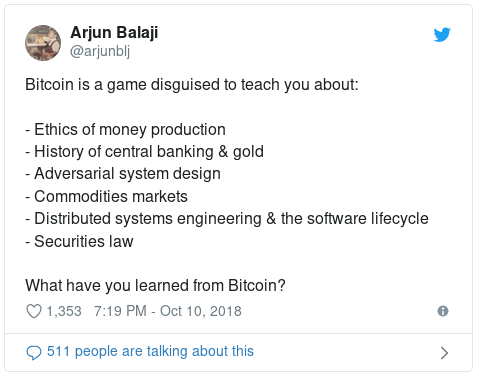
\includegraphics[width=7cm]{assets/images/the-tweet.png}
\end{center}

The \textit{21 Lessons} are structured in bundles of seven, resulting in three
chapters. Each chapter looks at Bitcoin through a different lens, extracting
what lessons can be learned by inspecting this strange network from a different
angle.

\paragraph{\hyperref[ch:philosophy]{Chapter 1}}{explores the philosophical
teachings of Bitcoin. The interplay of immutability and change, the concept of
true scarcity, Bitcoin's immaculate conception, the problem of identity, the
contradiction of replication and locality, the power of free speech, and the
limits of knowledge.
}

\paragraph{\hyperref[ch:economics]{Chapter 2}}{explores the economic teachings
of Bitcoin. Lessons about financial ignorance, inflation, value, money and the
history of money, fractional reserve banking, and how Bitcoin is re-introducing
sound money in a sly, roundabout way.}

\paragraph{\hyperref[ch:technology]{Chapter 3}}{explores some of the lessons
learned by examining the technology of Bitcoin.  Why there is strength in
numbers, reflections on trust, why telling time takes work, how moving slowly
and not breaking things is a feature and not a bug, what Bitcoin's creation can
tell us about privacy, why cypherpunks write code (and not laws), and what
metaphors might be useful to explore Bitcoin's future.}

~

Each lesson contains several quotes and links throughout the text. If an idea is
worth exploring in more detail, you can follow the links to related works in the
footnotes or in the bibliography.

Even though some prior knowledge about Bitcoin is beneficial, I hope that these
lessons can be digested by any curious reader. While some relate to each other,
each lesson should be able to stand on its own and can be read independently. I
did my best to shy away from technical jargon, even though some domain-specific
vocabulary is unavoidable.

I hope that my writing serves as inspiration for others to dig beneath the
surface and examine some of the deeper questions Bitcoin raises. My own
inspiration came from a multitude of authors and content creators to all of whom
I am eternally grateful.

Last but not least: my goal in writing this is not to convince you of anything.
My goal is to make you think, and show you that there is way more to Bitcoin
than meets the eye. I can’t even tell you what Bitcoin is or what Bitcoin will
teach you. You will have to find that out for yourself.

\begin{quotation}\begin{samepage}
\enquote{After this, there is no turning back. You take the blue pill --- the
story ends, you wake up in your bed and believe whatever you want to
believe. You take the red pill\footnote{the \textit{orange} pill} --- you stay in Wonderland, and I show
you how deep the rabbit hole goes.}
\begin{flushright} -- Morpheus
\end{flushright}\end{samepage}\end{quotation}

\begin{figure}
  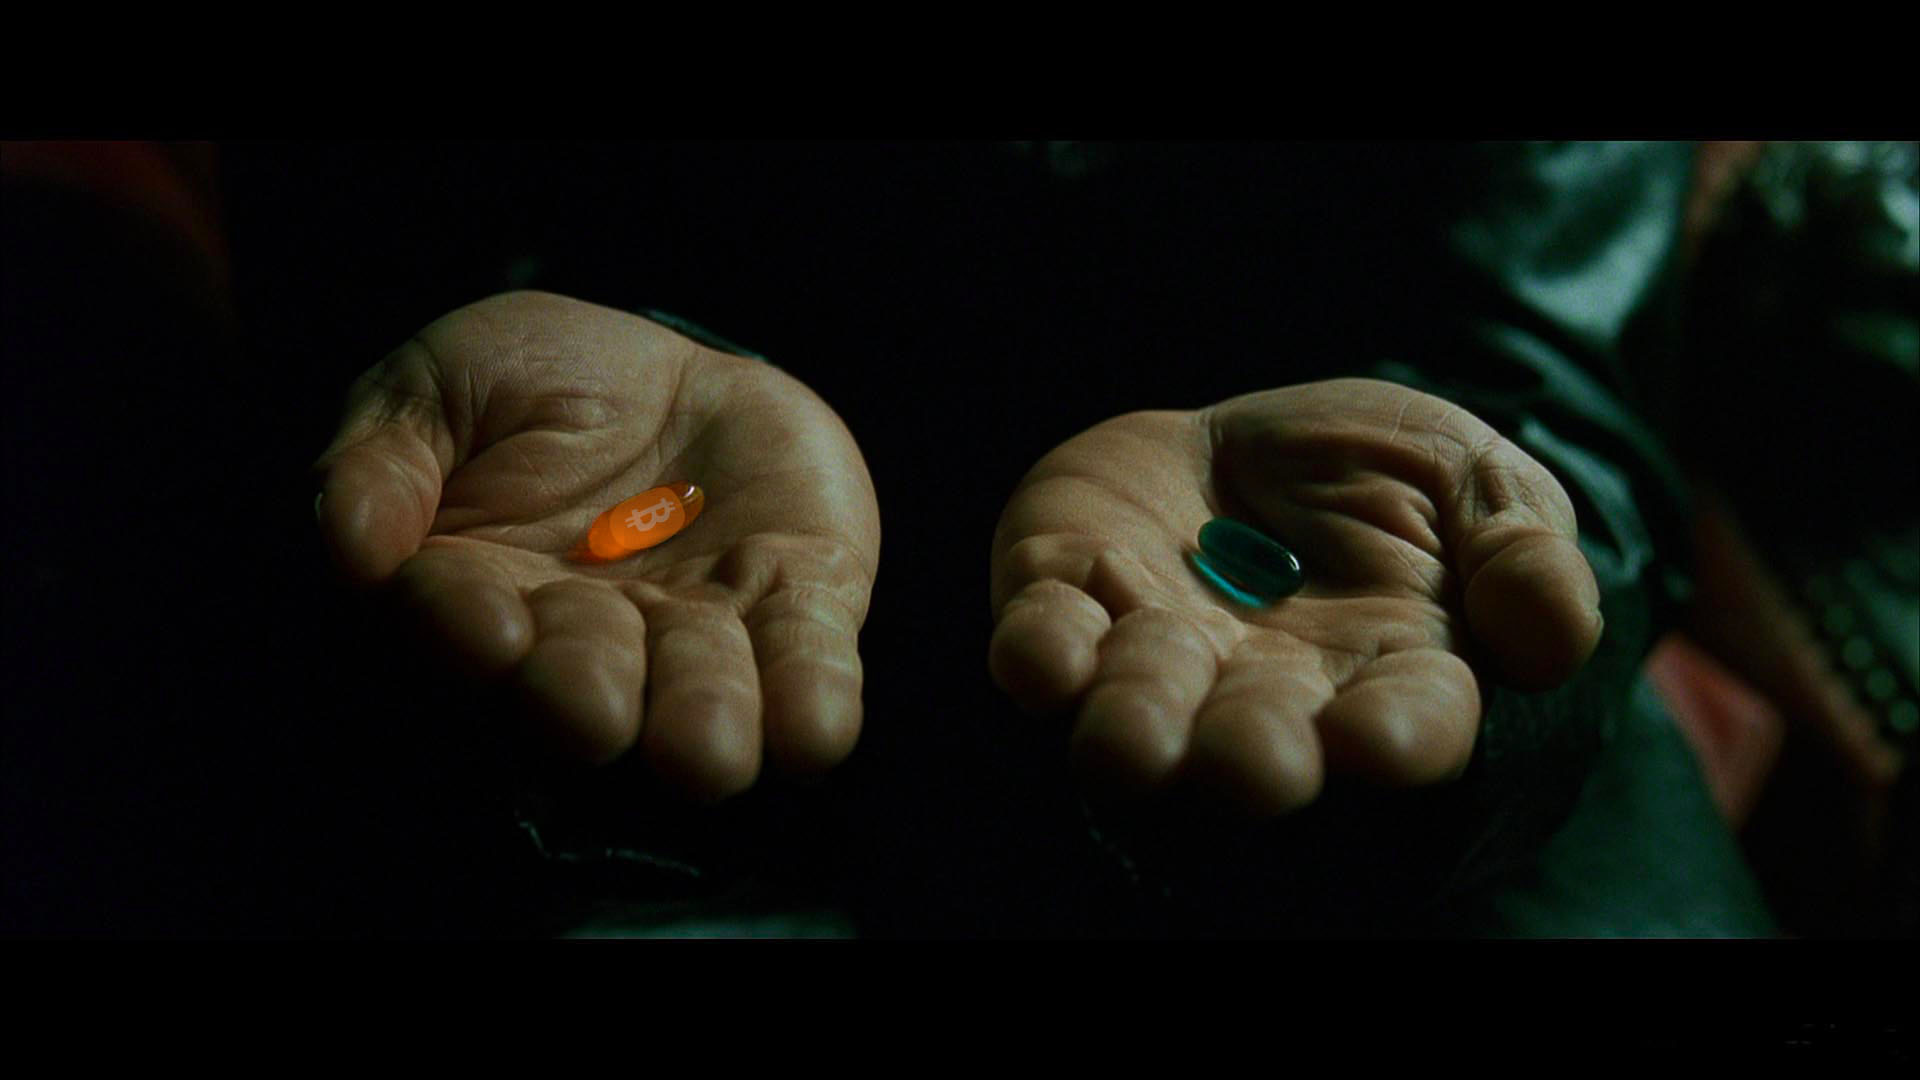
\includegraphics{assets/images/bitcoin-orange-pill.jpg}
  \caption*{Remember: All I'm offering is the truth. Nothing more.}
  \label{fig:bitcoin-orange-pill}
\end{figure}

%
% [Morpheus]: https://en.wikipedia.org/wiki/Red_pill_and_blue_pill#The_Matrix_(1999)
% [this question]: https://twitter.com/arjunblj/status/1050073234719293440
%
% <!-- Internal -->
% [chapter1]: {{ 'bitcoin/lessons/ch1-00-philosophy' | absolute_url }}
% [chapter2]: {{ 'bitcoin/lessons/ch2-00-economics' | absolute_url }}
% [chapter3]: {{ 'bitcoin/lessons/ch3-00-technology' | absolute_url }}
%
% <!-- Wikipedia -->
% [alice]: https://en.wikipedia.org/wiki/Alice%27s_Adventures_in_Wonderland
% [carroll]: https://en.wikipedia.org/wiki/Lewis_Carroll
